\question 

\begin{figure}[ht]
    \centering
    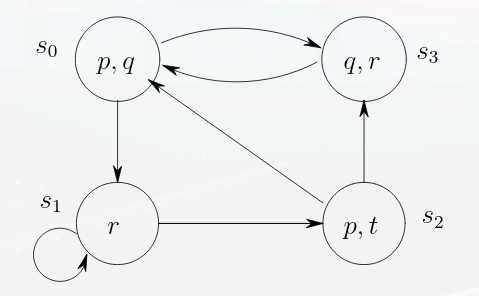
\includegraphics[width=0.35\textwidth]{fig/q4ts.png}
    \caption{The model}
    \label{fig:q4ts}
\end{figure}

\begin{alphaparts}
    \questionpart $\always\finally q$ --- $\model, s_0 \models \phi,\; \model, s_2 \models \phi$ 
    
    \questionpart $\always\globally \eventually\finally (p \lor r)$ --- $\model, s_0 \models \phi,\; \model, s_2 \models \phi$ 
    
    \questionpart $\eventually\lnext\eventually\lnext r$ --- $\model, s_0 \models \phi,\; \model, s_2 \models \phi$ 
    
    \questionpart $\always\globally\always\finally q$ --- $\model, s_0 \not\models \phi,\; \model, s_2 \not\models \phi$ 
    
    Consider the paths from each of the states that end up looping in $s_1$.
\end{alphaparts}